\documentclass[10pt]{beamer}

%STANDARD PREAMBLE
%https://tex.stackexchange.com/questions/68821/is-it-possible-to-create-a-latex-preamble-header
\usepackage{/Users/miw267/Repos/latex_preamble/beamer_preamble}
%\usepackage{/Users/miw267/Repos/csci246_spring2025/slides/preambles/beamer_preamble_for_CSCI246}


%%%
% SPECIFIC TO THIS DOCUMENT 
%%%
\usepackage{animate}

\renewcommand{\ELBO}{\texttt{ELBO}}
\renewcommand{\Q}{\mathcal{Q}}


%%%%
% DOCUMENT 
%%%
\title{04/21/2026: Diffusion with Transformers}
\author{Reference: \textit{Scalable Diffusion Models with Transformers}}
\date{CSCI 546: Diffusion Models}

\begin{document}
\maketitle

%\begin{frame}{Table of contents}
%  \setbeamertemplate{section in toc}[sections numbered]
%  \tableofcontents[hideallsubsections]
%\end{frame}

\begin{frame}{Table of contents}
  \setbeamertemplate{section in toc}[sections numbered]
  \setbeamertemplate{subsection in toc}[subsections numbered]
  \tableofcontents
\end{frame}





\section{Course Logistics}




\begin{frame}{Reading Survey \#9}

After having read this paper, if you were constructing a diffusion model for images, which backbone would you use, and why?
\end{frame}




\section{Lightning Chat: Diffusion with Transformers}

\begin{frame}[standout]
\href{https://docs.google.com/presentation/d/1i_iHb4rMHTgZkleerdyryA8Hdn3mvqSSLZQNyTmujlg/edit?slide=id.g3e03092e772_0_27\#slide=id.g3e03092e772_0_27}{\underline{Lightning Chat}} 
\end{frame}



\section{Mini-Lecture: Diffusion with Transformers}

\begin{frame}{Convolutional Neural Networks (CNNs)}
\begin{figure} 
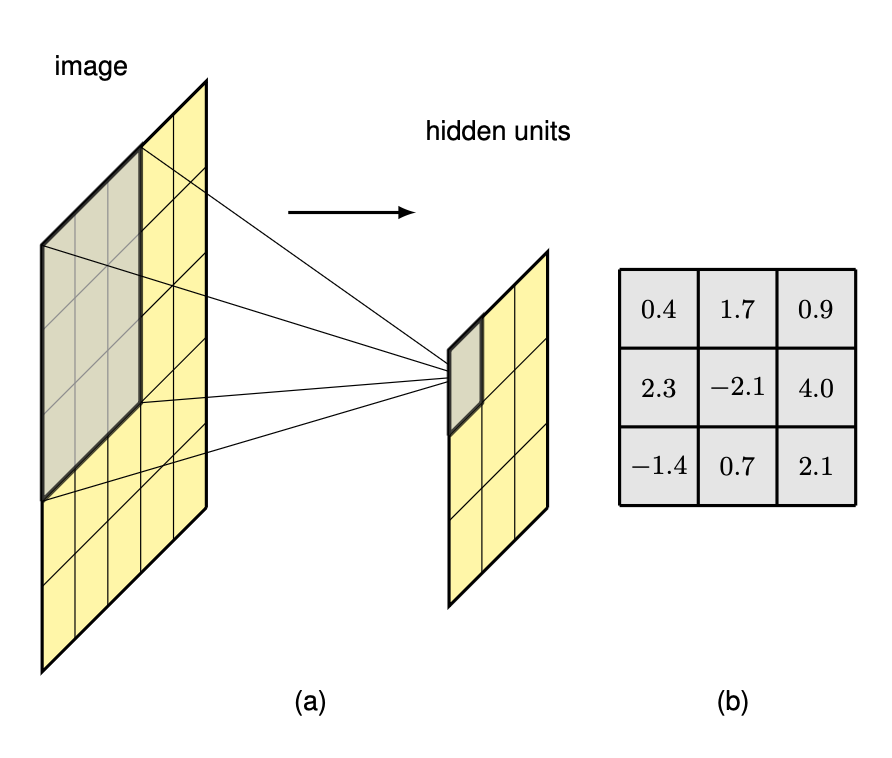
\includegraphics[width=.6\textwidth]{images/convolution_filter} 
\caption{A Convolution Filter \quad \tinytext{(Bishop, Deep Learning, pp.291)}}
\end{figure}

\only<2>{\colorbox{yellow!30}{\textbf{Poll.}} Who can explain what's going on here?}

\only<3>{\colorbox{blue!30}{\textbf{Remark.}} We use the \textbf{same} hidden-unit weights at multiple locations in the image.}
\end{frame}

\begin{frame}{Translation Invariance}

The CNN has an inductive bias for \alert{translation invariance} in classification.


\begin{figure}
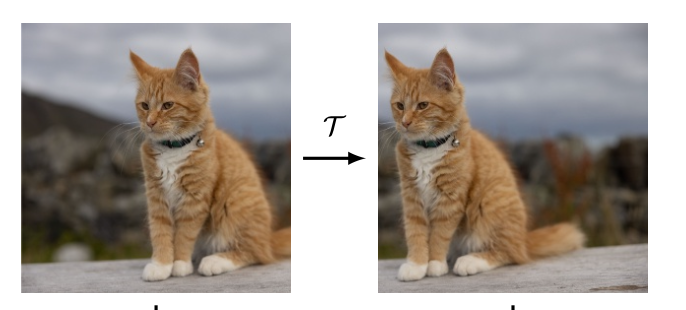
\includegraphics[width=.6\textwidth]{images/translation_invariance}  \\
\tinytext{(Bishop, Deep Learning, pp.260)}
\end{figure}

\vfill 
\pause 
If $\mathcal{C}$ is a neural network classifier,  $\mathcal{T}$ is a translation operator, and $\+I$ is an image, then we want
\[\mathcal{C}\big( \mathcal{T}(\+I) \big) =  \mathcal{C}\big( \+I \big)\] 

\end{frame}


\begin{frame}{Translation Equivariance}

The CNN also has an inductive bias for \alert{translation equivariance} for segmentation.

\begin{figure}
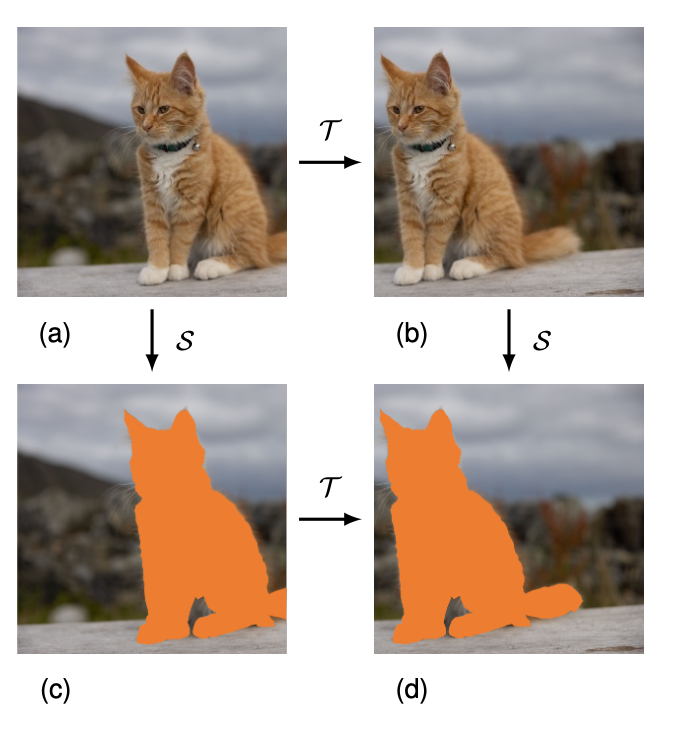
\includegraphics[width=.4\textwidth]{images/translation_equivariance}  \\
\tinytext{(Bishop, Deep Learning, pp.260)}
\end{figure}

\vfill 

If $\mathcal{S}$ is a segmentation network,  $\mathcal{T}$ is a translation operator, and $\+I$ is an image, then we want
\[\mathcal{S}\big( \mathcal{T}(\+I) \big) =  \mathcal{T}\big( \mathcal{S}(\+I) \big) \] 

\end{frame}

\begin{frame}{Vision Transformers}

The surprise of vision transformers (ViT) is that the \alert{inductive biases} induced by the CNN model architecture become \textbf{unnecessary} for modeling images at sufficiently large scales.

\begin{figure}
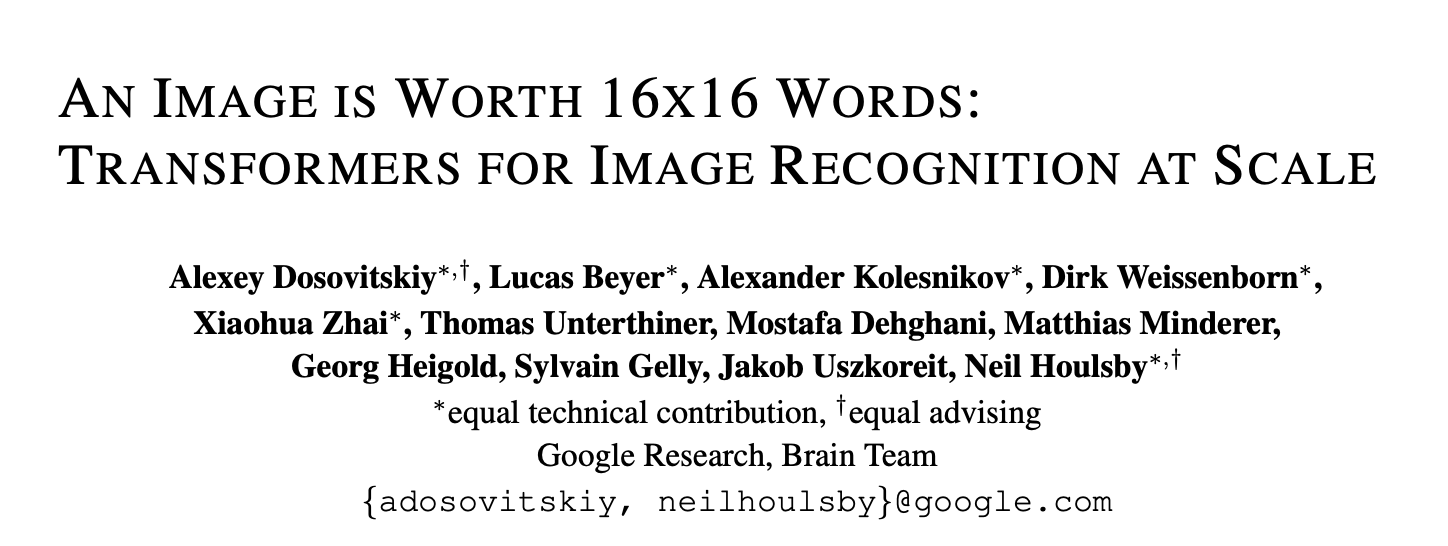
\includegraphics[width=\textwidth]{images/image_is_worth}  
\end{figure}

\end{frame}


\begin{frame}{Vision Transformers: How They Work}


\colorbox{yellow!30}{\textbf{Poll.}} But transformers operate on linear 1D sequence of tokens.  How do we apply it to 2D images?

\vfill 
\pause 

\begin{figure}
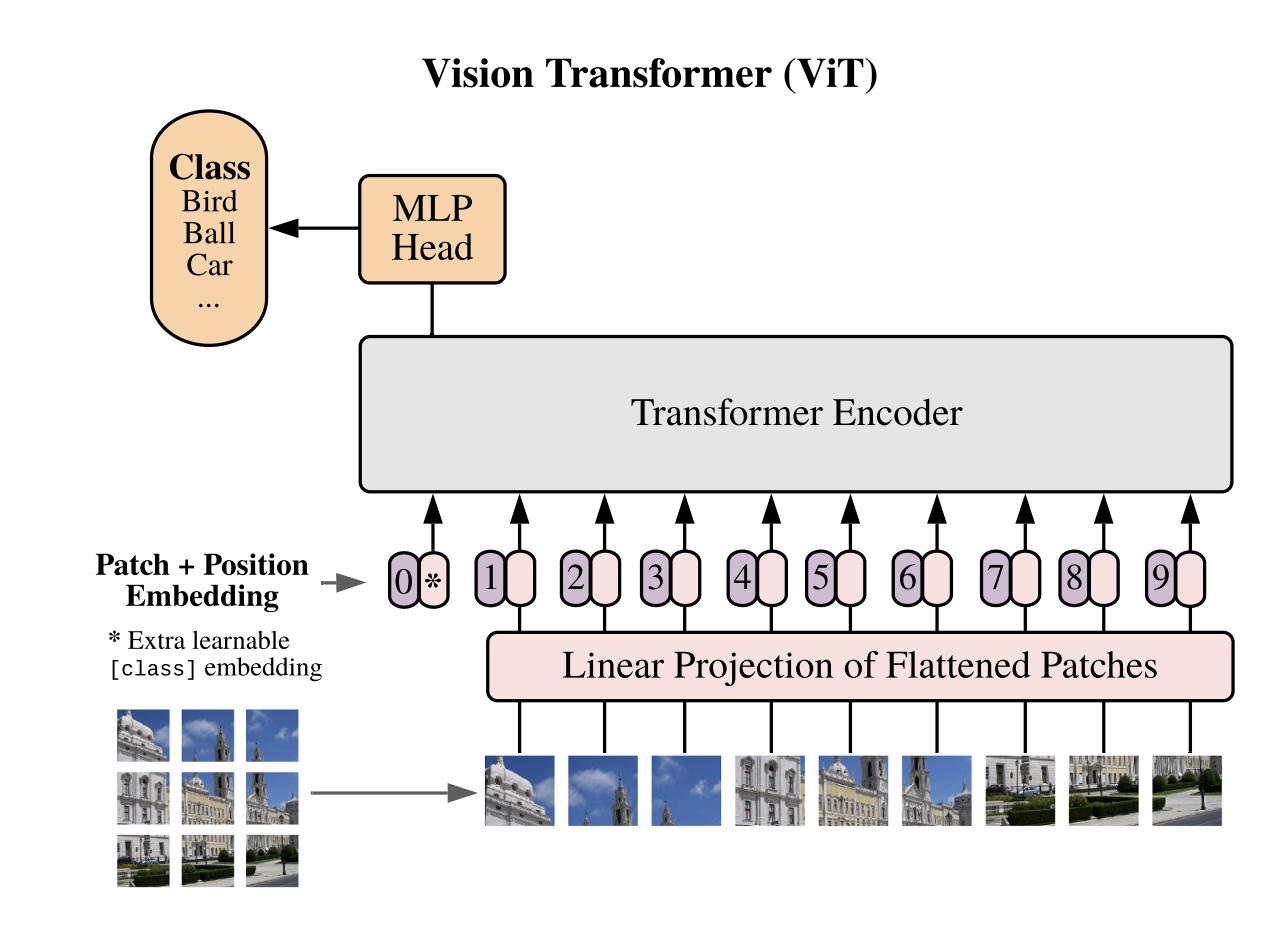
\includegraphics[width=.8\textwidth]{images/ViT}  
\end{figure}

\bottomtext{\hfill Reference: An image is worth 16x16 words.}
\end{frame}

\begin{frame}{Vision Transformers for Classification: The Role of Attention}


The model attends to regions that are semantically relevant for classification.

\begin{figure}
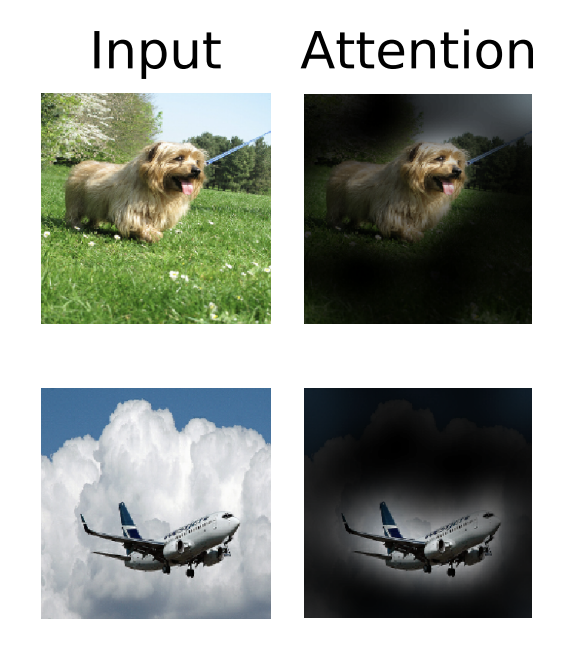
\includegraphics[width=.4\textwidth]{images/ViT_attention}
\caption{Representative examples of attention from the output token to the input space.}  
\end{figure}

\bottomtext{\hfill Reference: An image is worth 16x16 words.}
\end{frame}


\begin{frame}{Vision Transformers in Diffusion}


Diffusion models with ViT backbone make good generative models, as large as the model capacity is sufficiently large.

\begin{figure}
\includegraphics[width=.6\textwidth]{images/better_samples_from_scale}
\caption{\textit{Increasing transformer Gflops increases sample quality.} Increasing the Gflops - either by increasing transformer depth/width or increasing the number of input tokens - yields significant improvements in visual fidelity.}
\end{figure}

\bottomtext{\hfill Reference: Scalable Diffusion Models With Transformers.}
\end{frame}


\begin{frame}{Relevance to final project}

\colorbox{yellow!30}{\textbf{Poll.}} So should anyone doing image generation use ViT instead of UNets as the backbone for their diffusion model?

\pause 
\vfill 
\begin{quotation}
When trained on mid-sized datasets such as ImageNet [1M images], these models yield modest accuracies [...] This seemingly discouraging outcome may be expected: Transformers lack some of the inductive biases inherent to CNN's, such as translational equivariance and locality [...] However, the picture changes if the models are trained on larger datasets (14M-300M images). We find that large scale training trumps inductive bias. 
\vspace{0.5em} \\
\hfill --- \textnormal{An image is worth 16x16 words.}

\end{quotation}
\end{frame}

\begin{frame}{Final project: General leads about diffusion modeling}

\colorbox{blue!30}{\textbf{Remark.}} Between 2020-2023, the following led to improvements in diffusion modeling (of images):

\begin{itemize}
	\item Predicting the noise \greencheck \pause 
	\item Latent diffusion models  \pause 
	\item Classifier-free guidance 
	\item Cascaded diffusion models 
\end{itemize}

\bottomtext{\hfill Reference: Scalable Diffusion with Transformers, pp. 4197-4198}
\end{frame}







\section{Coding Workshop On Attention: Part II}

\begin{frame}{Complete Coding Workshop}
\begin{itemize}
\item \href{https://docs.google.com/presentation/d/1_SY-tAbZFY8irih9neKzLfv3miCtsh4p9bxCeoW896U/edit?usp=sharing}{\underline{\blue{Sam and Dillon}}}
\item \href{https://docs.google.com/presentation/d/1Ej1u6c1l3iVIl6_jghKfbHAgqC1-_A8fWtkO_3l_5CE/edit?usp=sharing}{\underline{\blue{Owen}}}
\item \href{https://montanaedu-my.sharepoint.com/:b:/g/personal/t83h237_student_montana_edu/IQAxz5FhInYzSKwS3QhA2V5PASBKxF55_T7uX-_qB83dDtw}{\underline{\blue{Matt}}}	
\end{itemize}


\end{frame}




\section{Mini-Lecture: Attention}

\begin{frame}[standout]
See previous slide deck
\end{frame}


\end{document}

